\section{Résultats de l'allocation proposée par DeepSeek}\label{sec:resultats-allocation}

Le protocole de la section~\ref{sec:protocole-allocation} permet cette fois à la réponse du modèle de modifier un portefeuille simulé. Les résultats du tableau~\ref{tab:allocation-performance} portent sur mai 2021--décembre 2025, à partir de 100 unités au 30 avril 2021. Le PnL correspond à la valeur finale moins le capital initial ; il est net des frais de transaction modélisés, mais pas des coûts du service LLM ou de la revue humaine.

\begin{table}[H]
\centering
\caption{Performance de l'expérience d'allocation, mai 2021--décembre 2025.}
\label{tab:allocation-performance}
\small
\begin{tabular}{lrrr}
\toprule
\textbf{Indicateur} & \textbf{Équipondéré} & \textbf{Inverse vol.} & \textbf{DeepSeek} \\
\midrule
Capital final & 153,55 & 152,26 & 148,39 \\
PnL & +53,55 & +52,26 & +48,39 \\
Rendement annualisé & 9,62\,\% & 9,42\,\% & 8,82\,\% \\
Volatilité quotidienne annualisée & 15,66\,\% & 15,08\,\% & 14,87\,\% \\
Sharpe quotidien, taux sans risque nul & 0,667 & 0,674 & 0,645 \\
Drawdown maximal quotidien & -24,20\,\% & -23,44\,\% & -23,50\,\% \\
\bottomrule
\end{tabular}
\end{table}

Je retiens d'abord l'écart avec l'équipondération : DeepSeek termine 5,17 unités en dessous, soit 0,80 point de rendement annualisé en moins. Sa volatilité plus faible ne s'accompagne pas d'un meilleur Sharpe. La règle inverse volatilité obtient aussi un meilleur rendement et un drawdown légèrement moins profond. Ces comparaisons m'amènent à relativiser l'intérêt financier de la décision LLM sur cette expérience.

\begin{figure}[H]
\centering
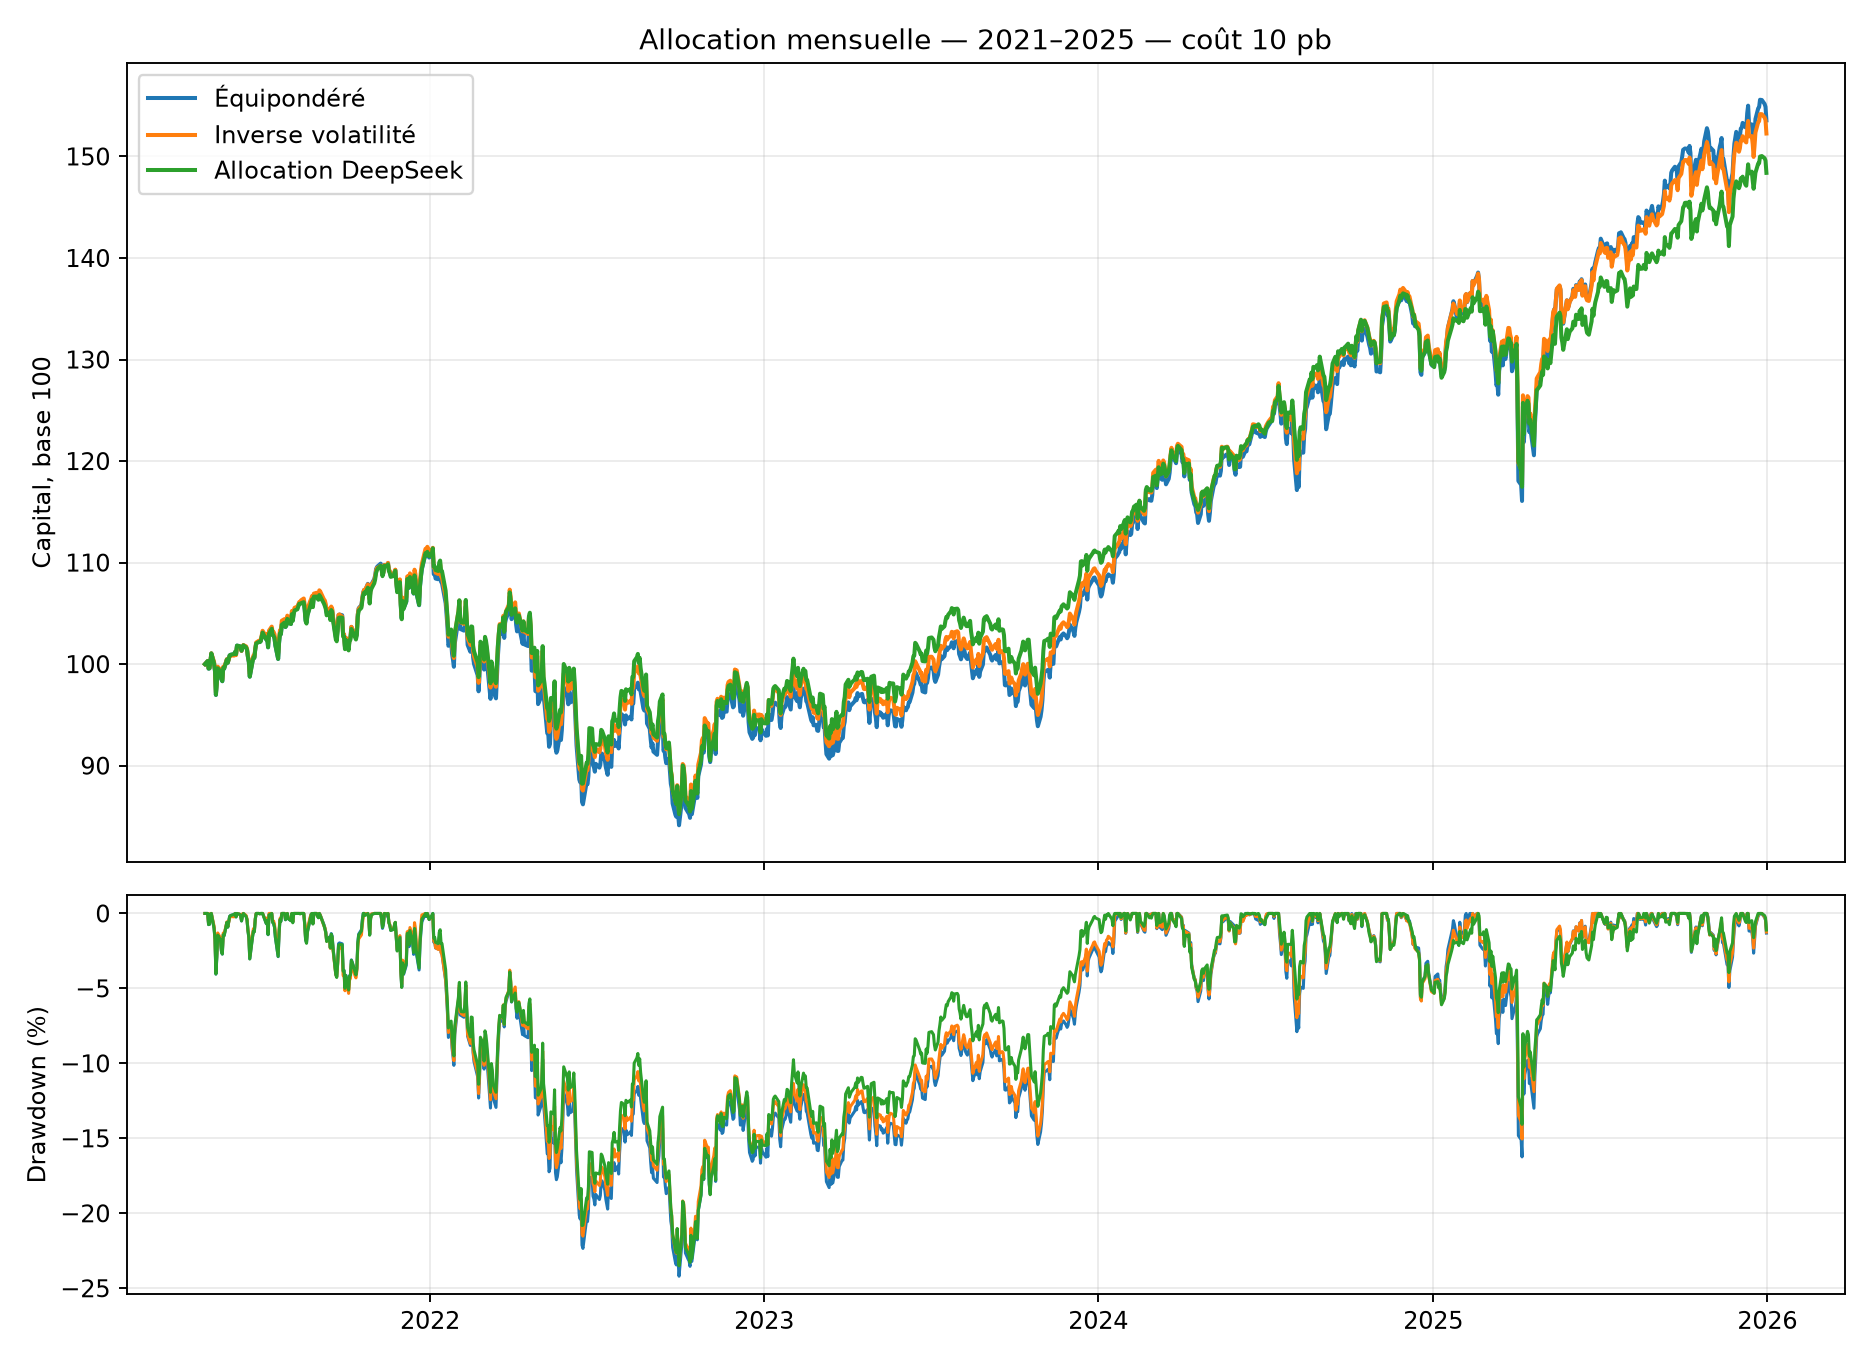
\includegraphics[width=0.98\textwidth]{figures/allocation_pnl_comparison.png}
\caption{Capital et drawdown des trois politiques d'allocation, de mai 2021 à décembre 2025. Frais de 10 pb par unité de turnover ; valeurs quotidiennes.}
\label{fig:allocation-pnl}
\end{figure}

\subsection{Variations selon les années}

\begin{table}[H]
\centering
\caption{Rendements nets par année de l'expérience d'allocation.}
\label{tab:allocation-annuel}
\small
\begin{tabular}{lrrr}
\toprule
\textbf{Période} & \textbf{Équipondéré} & \textbf{Inverse vol.} & \textbf{DeepSeek} \\
\midrule
2021, mai--décembre & 10,50\,\% & 11,14\,\% & 10,61\,\% \\
2022 & -15,51\,\% & -14,80\,\% & -14,84\,\% \\
2023 & 16,01\,\% & 15,36\,\% & 17,92\,\% \\
2024 & 19,47\,\% & 18,86\,\% & 16,59\,\% \\
2025 & 18,68\,\% & 17,26\,\% & 14,58\,\% \\
\bottomrule
\end{tabular}
\end{table}

Le classement n'est pas identique chaque année. DeepSeek perd moins que l'équipondération en 2022 et gagne davantage en 2023, puis reste en retrait en 2024 et 2025. Ces écarts décrivent la trajectoire obtenue ; ils ne prouvent pas que le modèle identifie correctement des régimes de marché. Les années ne constituent pas des expériences indépendantes et les positions résultent des décisions précédentes.

\subsection{Propositions reçues, exécutées et rejetées}

Les 56 réponses de la campagne corrigée sont reçues et décodées en JSON. Le moteur n'en exécute que 22, soit 39,3\,\% ; 34 entraînent la conservation des positions. Les deux références déterministes passent les 56 contrôles. Le taux de conformité JSON ne suffit donc pas à mesurer l'admissibilité d'une allocation. Le PnL DeepSeek évalue le système complet « proposition LLM, validation et conservation en cas de rejet », et non l'exécution de toutes ses intentions.

\begin{table}[H]
\centering
\caption{Motifs de rejet des propositions DeepSeek.}
\label{tab:allocation-rejets}
\small
\begin{tabular}{p{0.78\textwidth}r}
\toprule
\textbf{Motif} & \textbf{Occurrences} \\
\midrule
Turnover demandé supérieur à 10\,\% à l'observation & 31 \\
Turnover réellement échangé après frais supérieur à 10\,\% & 2 \\
Somme des poids différente de 1 & 1 \\
Poids hors limites & 1 \\
Référence à un champ absent des entrées & 1 \\
\bottomrule
\end{tabular}
\end{table}

Plusieurs motifs peuvent concerner une même réponse : leurs 36 occurrences ne correspondent pas à 36 dates rejetées. Le cas du 30 avril 2021 illustre la principale difficulté. Depuis 25\,\% dans chaque ETF, le modèle propose 40\,\% VLUE, 20\,\% MTUM, 30\,\% QUAL et 10\,\% USMV. Le turnover vaut alors :
\[
\frac{1}{2}\left(0{,}15+0{,}05+0{,}05+0{,}15\right)=0{,}20.
\]
La justification affirme pourtant respecter la limite de 10\,\%. Python rejette la proposition. Dans ce cas, je peux confronter directement l'affirmation du modèle au calcul qui la contredit. C'est l'apport du contrôle numérique indépendant ; l'admissibilité des 22 réponses acceptées laisse ouverte la question de leur raisonnement financier.

\subsection{Coûts de transaction et ressources du service LLM}\label{sec:couts-allocation}

\begin{table}[H]
\centering
\caption{Turnover exécuté et frais déduits des portefeuilles, capital initial 100.}
\label{tab:allocation-couts}
\small
\begin{tabular}{lrrr}
\toprule
\textbf{Indicateur} & \textbf{Équipondéré} & \textbf{Inverse vol.} & \textbf{DeepSeek} \\
\midrule
Turnover mensuel moyen & 0,752\,\% & 1,146\,\% & 1,188\,\% \\
Somme des frais, en unités de capital & 0,0476 & 0,0708 & 0,0682 \\
\bottomrule
\end{tabular}
\end{table}

Les mois rejetés ont un turnover nul dans cette moyenne. Le coût reste faible pour ce portefeuille limité à quatre ETF, avec des décisions mensuelles et de nombreux rejets. La somme des frais n'est pas la perte de richesse finale attribuable aux coûts : elle n'intègre pas leur capitalisation ultérieure. La différence de performance ne peut pas être décomposée rigoureusement en effet d'allocation et effet des frais sans un scénario contrefactuel supplémentaire. Les simulations LLM à 0 et 30 points de base n'ont pas été réalisées.

\begin{table}[H]
\centering
\caption{Ressources rapportées par l'API pendant la collecte d'allocation.}
\label{tab:allocation-api}
\small
\begin{tabular}{p{0.57\textwidth}rr}
\toprule
\textbf{Indicateur} & \textbf{Campagne} & \textbf{Essais techniques} \\
\midrule
Tentatives & 56 & 4 \\
Réponses avec usage reçu & 56 & 3 \\
Jetons d'entrée rapportés & 43\,263 & 2\,375 \\
Jetons de sortie rapportés & 11\,376 & 9\,000 \\
Total des jetons rapportés & 54\,639 & 11\,375 \\
Durée cumulée des réponses reçues & 86,02 s & 37,61 s \\
\bottomrule
\end{tabular}
\end{table}

La campagne représente 54\,639 jetons rapportés, auxquels s'ajoutent 11\,375 jetons des trois essais techniques terminés. Le total connu est donc de 66\,014 jetons ; l'usage de la quatrième tentative interrompue n'a pas été reçu et peut néanmoins avoir été facturé. La médiane des durées d'appel de la campagne est de 1,43 seconde, avec un maximum de 2,38 secondes. Ces mesures concernent les appels reçus, pas l'ensemble du temps de développement, de tests et d'analyse.

L'archive distingue 7\,040 jetons d'entrée servis depuis le cache et 36\,223 hors cache pour la campagne. Si $p_h$, $p_m$ et $p_s$ désignent les tarifs par million de jetons d'entrée en cache, hors cache et de sortie, son coût théorique est :
\[
C_{\mathrm{API}}=\frac{7\,040p_h+36\,223p_m+11\,376p_s}{10^6}.
\]
Ce montant doit être complété par les essais techniques et rapproché de la facture du fournisseur. Aucun montant en euros ou en dollars n'est présenté comme un coût observé : les archives ne contiennent pas le tarif effectivement facturé ni le relevé de compte. Appliquer rétrospectivement un tarif affiché ne remplacerait pas cette preuve.

Les dépenses API, l'infrastructure, le développement et la revue humaine sont exclues des valeurs de portefeuille. Le temps d'analyse humaine et le coût des données n'ont pas été mesurés. La base 100 est une unité normalisée, sans capital monétaire fixé : une facture réelle ne peut donc pas être soustraite directement de ce PnL. Pour un capital initial réel $K$, un coût externe $C$ payé à l'échéance représenterait $100C/K$ unités de cette base ; des paiements intervenant plus tôt demanderaient de simuler les flux et leur effet sur les positions. Le coût total d'exploitation reste ainsi à établir.

\subsection{Vérifications obtenues}

Les 46 tests du projet réussissent, dont 23 ajoutés pour l'allocation. Ils couvrent notamment l'invariance des entrées aux cours futurs, l'exécution différée, la conservation des quantités après rejet, les frais à 0, 10 et 30 points de base et la conservation du capital. Une politique produisant exactement les poids équipondérés donne exactement le même PnL que cette référence.

Les 56 décisions ont ensuite été rejouées hors réseau : les fichiers des valeurs, des métriques et des décisions sont identiques octet par octet, sans nouvel appel API. Un contrôle indépendant à partir des positions et des prix a vérifié 3\,519 valorisations quotidiennes, soit 1\,173 séances pour chacune des trois politiques. L'erreur maximale observée est de $5{,}68\times10^{-14}$ unité. Les 31 fichiers antérieurs couverts par le contrôle SHA-256 sont demeurés inchangés lors de cette extension. Ces vérifications établissent la cohérence du calcul observé ; elles ne valident pas les hypothèses de marché.

\subsection{Biais et portée de l'interprétation}\label{sec:biais-allocation}

\paragraph*{Information future et préentraînement.}
La coupure des séries protège les indicateurs transmis au modèle. Le service appelé en septembre 2026 peut cependant avoir appris des événements de 2021--2025 pendant son préentraînement ; la date et les tickers restent visibles. Cette simulation historique ne constitue donc pas une évaluation prédictive hors échantillon du LLM. Le replay reproduit des décisions connues, sans tester ce que le modèle aurait décidé avec les seules connaissances disponibles à l'époque.

\paragraph*{Données et sélection de l'univers.}
Les cours ajustés utilisés aujourd'hui ne sont pas archivés dans leur version disponible à chaque date historique. Les ajustements et événements sur titres n'ont pas fait l'objet d'une validation indépendante exhaustive. Quatre ETF américains existants ont été choisis ; le résultat ne mesure ni le biais de survie ni les effets de sélection qu'introduirait un univers plus large. Les quatre expositions restent des proxies ETF, avec leurs règles et coûts propres, et non des facteurs reconstruits titre par titre.

\paragraph*{Choix du protocole et dépendance au modèle.}
La période de 56 mois résulte de l'incident technique et du budget, pas d'un tirage indépendant. Les horizons d'indicateurs, le prompt, les plafonds de 40\,\% et 10\,\% et les références sont des choix expérimentaux ; ils n'ont pas été optimisés sur le PnL de cette campagne. Leurs alternatives n'ont pas été comparées. Les modèles et paramètres de service peuvent évoluer, et une seule réponse par date ne permet pas de mesurer la dispersion entre répétitions. Aucune sélection a posteriori d'une meilleure trajectoire n'a été effectuée.

\paragraph*{Effet des rejets et validité économique.}
Les 34 conservations de positions influencent fortement le portefeuille. La performance ne peut pas être attribuée au seul choix économique du modèle : elle combine ce choix, les contraintes et la règle de repli. Même une citation exacte ne démontre pas que l'indicateur justifie l'allocation. Aucun test de significativité, attribution factorielle, ajustement du risque de benchmark ou protocole prospectif ne permet ici de conclure à un alpha.

\paragraph*{Écart avec l'exploitation réelle.}
L'exécution à la clôture suivante est une convention de simulation. Les frais fixes ne représentent pas un carnet d'ordres, des spreads variables, des contraintes de capacité ou de fiscalité. Les poids peuvent dériver après transaction, le portefeuille est supposé déjà investi et les coûts de sortie ne sont pas inclus. Enfin, l'acceptation par Python n'enregistre pas une approbation humaine et ne donne aucune permission d'ordre réel.

J'en retiens un résultat technique et un résultat financier distincts : la chaîne transforme des propositions LLM en positions vérifiables et bloque des erreurs observées ; elle sous-performe ici les références simples. Une suite utile serait de faire choisir le modèle parmi des allocations déjà admissibles, puis de comparer ce choix à une règle déterministe alimentée par les mêmes indicateurs, dans une nouvelle expérience définie avant examen des rendements.
